\documentclass[AutoFakeBold,AutoFakeSlant]{beamer}

\usepackage[british]{babel}
\usepackage{graphicx,hyperref,sysu,url}

%% 中文
\usepackage{ctex}

\usepackage{newtxmath}
\RequirePackage{booktabs}
\usepackage{multicol} 
\usepackage{multirow}
\usepackage[ruled,linesnumbered]{algorithm2e}
\usepackage{color}

% colors
\definecolor{sysugreen}{RGB}{0,88,38}
\definecolor{sysugreendark}{RGB}{5,71,25}

% commands
\newcommand{\ctoday}{\number\year 年 \number\month 月 \number\day 日}

%% 根据需要修改中文字体
\setCJKmainfont[ItalicFont={SimSun}]{SimSun}
% \setCJKsansfont{Microsoft YaHei}
\setCJKsansfont{SimHei}
\setCJKmonofont{FangSong}

% \setCJKmonofont{SimSun}
% \xeCJKsetcharclass{"0}{"2E7F}{0}
% \xeCJKsetcharclass{"2E80}{"FFFF}{1}

% Require XeLaTeX
\RequirePackage{fontspec,xltxtra,xunicode}
% 根据需要修改英文字体
\setmainfont[Mapping=tex-text]{Times New Roman}
\setsansfont[Mapping=tex-text]{Arial}
\setmonofont{Consolas}

% 设置公式字体
\usefonttheme[onlymath]{serif}


% 演示文稿标题:
%  1 底部显示的标题;
%  2 标题页正中显示的大标题;
\title[中山大学硕士学位论文答辩]{
  大标题}

% 可选:标题页显示的副标题
\subtitle{副标题}

% 作者信息:
%  1 底部显示的作者信息;
%  2 联系信息;
% \author[Author Name]{
%   答辩人 \\\medskip
%   {\small \url{netid@mail2.sysu.edu.cn}} \\
%   {\small \url{www.sysu.edu.cn}}
% }

% 学校学院信息:
%  1 顶部学校信息
%  2 标题页显示的学院学校信息
\institute[Sun Yat-Sen University]{
  XX学院 \\ 
  中山大学}

%% 时间信息
%  1 底部显示的标准时间信息
%  2 标题页显示的中文时间信息
\date[\today]{\ctoday}


\begin{document}

% 作者信息
\author[Author Name]{
  答辩人 
  \texorpdfstring{\\\medskip {\small xxxx专业}}{}
  \texorpdfstring{\\ {\small 导师~xxx教授}}{}
}

\begin{frame}
  % 标题页
  \titlepage
\end{frame}
% 标题页不编号
\setcounter{framenumber}{0}

\begin{frame}
  % 目录页
  \frametitle{目\quad 录}
  % 双栏
  % \begin{multicols}{2}
  %   \tableofcontents
  % \end{multicols}
  \tableofcontents[hideallsubsections]
\end{frame}

\section{引言}

\begin{frame}
  \frametitle{介绍}

  \begin{itemize}
    \item 修改自人大模板Latex beamer template for RUC\footnote{\url{https://github.com/andelf/ruc-beamer-template}}
    \begin{itemize}
      \item 基于“\textcolor{sysugreen}{中大绿}”颜色 \footnote{\url{http://www.sysu.edu.cn/}}
      \item Logo等取自中山大学视觉形象识别系统
    \end{itemize}
  \end{itemize}
\end{frame}

\begin{frame}
  \frametitle{内容}

  引言内容包括:
  \begin{enumerate}
    \item \textbf{本研究课题的学术背景及理论与实际意义};
    \item \textbf{本研究课题的来源及主要研究内容};
    \item \textbf{建立研究的线索与思路}。
  \end{enumerate}

\end{frame}

\section{研究现状}

\subsection{区块}

\begin{frame}
  \frametitle{普通区块}

  \begin{block}{国内\LaTeX\ 讨论区}
    \begin{enumerate}
      \item LaTeX Studio\footnote{\url{https://www.latexstudio.net/}}
    \end{enumerate}
  \end{block}

  \begin{block}{国外\LaTeX\ 讨论区}
    \begin{enumerate}
      \item LaTeX Stack Exchange\footnote{\url{https://tex.stackexchange.com/}}
    \end{enumerate}
  \end{block}
\end{frame}

\begin{frame}
  \frametitle{其他区块}

  \begin{theorem}{theorem 定理环境}

  \end{theorem}

  \begin{lemma}{lemma 引理环境}
    
  \end{lemma}

  \begin{proof}{proof 证明环境}
    
  \end{proof}
\end{frame}

\begin{frame}
  \frametitle{其他区块}

  \begin{corollary}{corollary 推论环境}
    
  \end{corollary}

  \begin{example}{example 示例环境}
    
  \end{example}

  \begin{alertblock}{alertblock 警示环境}

  \end{alertblock}
\end{frame}

\section{研究方法}

\subsection{步骤一}

\begin{frame}
  \frametitle{公式}
  行内公式$\boldsymbol{\theta}\in\mathbb{R}^{h}$,行间公式:
  \begin{equation}
    \theta_{i}\leftarrow\theta_{i}-\alpha\frac{\partial J(\theta)}{\partial\theta_{i}}
  \label{equ}
  \end{equation}
\end{frame}

\subsection{步骤二}

\begin{frame}
  \frametitle{算法}

  \begin{algorithm}[H]
  \footnotesize
  \KwIn{训练数据$\mathcal{D}$}
  \KwOut{参数$\theta$}
  \Repeat{收敛}{
      根据公式\ref{equ}迭代更新\;
  }
  \caption{本研究提出算法}
  \label{algo}
  \end{algorithm}
\end{frame}

\section{实例验证}

\subsection{实验设计}
\begin{frame}
  \frametitle{数据集}

  \begin{itemize}
    \item 实验数据集:规模、时间跨度、区域。
  \end{itemize}
\end{frame}

\begin{frame}
  \frametitle{实验环境}

  \begin{itemize}
    \item 计算环境:Intel i7-9700K,16GB RAM,RTX 2070 super
    \item 编程环境:PyTorch 1.4
  \end{itemize}
\end{frame}

\subsection{实验结果与讨论}

\begin{frame}
  \frametitle{实验结果}

  \begin{table}[ht]
  \footnotesize
  \caption{不同模型实验结果对比}
  \centering
  \begin{tabular}{clcc}
  \toprule
  \multicolumn{2}{c}{\textbf{模型}} & \textbf{指标1} & \textbf{指标2} \\
  \midrule
  \multicolumn{2}{c}{Baseline1} & 0.889 & 0.909 \\
  \multicolumn{2}{c}{Baseline2} & 0.901 & 0.921 \\
  \multicolumn{2}{c}{Baseline3} & 0.922 & 0.913 \\
  \midrule
  \multirow{3}{*}{本文模型} & $\lambda=10$ & 0.921 & 0.934 \\
  & $\lambda=20$ & 0.928 & 0.932 \\
  & $\lambda=50$ & 0.927 & 0.940 \\
  \bottomrule
  \end{tabular}
  \label{result}
  \end{table}
\end{frame}

\begin{frame}
  \frametitle{讨论}
  页内分栏:
  \begin{columns}

  \column{.5\textwidth}
  \begin{figure}
    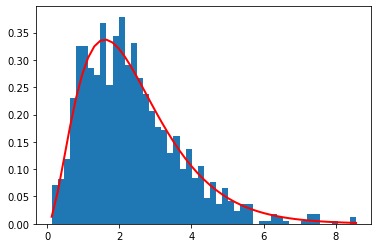
\includegraphics[width=\textwidth]{image/result1.png}
    \caption{$\alpha=2.98, \beta=\frac{1}{1.24}$}
    \label{fig1}
  \end{figure}
  
  
  \column{.5\textwidth}
  \begin{figure}
    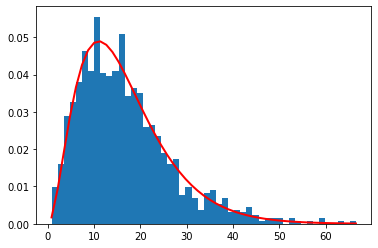
\includegraphics[width=\textwidth]{image/result2.png}
    \caption{$\alpha=2.98, \beta=\frac{1}{0.18}$}
    \label{fig2}
  \end{figure}
  
  \end{columns}

\end{frame}

\section{结论}

\subsection{工作总结}
\begin{frame}
  \frametitle{工作总结}

  \begin{enumerate}
    \item 本文提出XXX。
  \end{enumerate}
\end{frame}

\subsection{研究展望}
\begin{frame}
  \frametitle{研究展望}

  \begin{enumerate}
    \item 针对问题XXX。
  \end{enumerate}
\end{frame}

\section{}
\begin{frame}[plain]
  
    \LARGE{
    感谢您的聆听。\\
    请老师们批评指正!}
  
\end{frame}

\end{document}
